\documentclass[10pt,openany]%,oneside]
{book}
\newcommand{\versiondate}[0]{February 5th, 2021}

%comment these two lines out to revert to default font
\usepackage{kpfonts}
\usepackage[T1]{fontenc}
\usepackage{inconsolata}

\usepackage{
  amsmath, calc,
  caption, changepage,
  endnotes, enumerate,
  epstopdf,
  fancyhdr,
  fix-cm,
  fncychap,
  footmisc,
  fullminipage,
  geometry, graphicx,
  ifthen, lscape,
  makeidx, manfnt,
  marginnote,
  mdframed,
  multicol, multirow,
  setspace, soul,
  tabto,
  textcomp,
  varioref, verbatim,
  wasysym, wrapfig
}
%\usepackage[usenames,dvipsnames]{color, colortbl}
\usepackage{color, colortbl}
\usepackage[explicit]{titlesec}
\usepackage{imakeidx, titlesec, paralist, qtree}%
\usepackage{subfigure}


\include{extraTeX/style/colorsV1}

% _____ Online Version _____ %
\usepackage[bookmarksnumbered, colorlinks = false, pdfborder = {0 0 0}, urlcolor = oiGB, colorlinks=true, linkcolor = oiGB, citecolor = oiGB, backref = true]{hyperref}
\newcommand{\printlocation}[0]{}

% _____ Print Version _____ %
%\definecolor{oiB}{rgb}{0,0,0}\definecolor{chaptertitlegray}{rgb}{0,0,0}\usepackage[colorlinks=false,pdfborder={0 0 0},urlcolor= black,colorlinks=black,linkcolor=black, citecolor=black,backref=true]{hyperref}


% _____ COLOR PRINT Version _____ %
%\usepackage[colorlinks=false,pdfborder={0 0 0},urlcolor= black,colorlinks=black,linkcolor=black, citecolor=black,backref=true]{hyperref} %\renewcommand{\printlocation}[0]{\noindent Printed in China. \\}

\definecolor{lightturquoise}{rgb}{0.25,0.88,0.82}


\def\labelitemi{--}
\setstretch{1.1}
  
\usepackage[style=authortitle-ibid, maxnames=2,natbib=true,sortcites=true,block=space,backend=bibtex]{biblatex}
\usepackage{fnpct}
\AdaptNoteOpt\footfullcite\multfootcite

\newenvironment{problem}[1][]{\relax \par \bigskip  \qt{Exercise} \eoce\relax\relax}{}
\bibliography{eoce.bib}

\makeindex 
% 1 Page Parameters
% 2 Special Commands for Editions
% 3 Content Modifications
% 4 Counters and Parameters
% 5 Section Coloring
% 6 Utilities
% 7 
% 8 Figures and Captions
% 9 Examples and Exercises
% 10 Special Boxes

%\renewcommand\chapter{\if@openright\cleardoublepage\else\clearpage\fi
%                    \thispagestyle{fancy}%
%                    \global\@topnum\z@
%                    \@afterindentfalse
%                    \secdef\@chapter\@schapter}
\fancypagestyle{plain}{%
\fancyhf{} % clear all header and footer fields
\fancyhead[RO,RE]{\thepage} %RO=right odd, RE=right even
\renewcommand{\headrulewidth}{0pt}
\renewcommand{\footrulewidth}{0pt}}
\raggedbottom


\newcommand{\stdspace}[0]{3mm}
\newcommand{\stdvspace}[0]{\vspace{\stdspace{}}}
\newcommand{\stdaddvspace}[0]{\addvspace{\stdspace{}}}




%-------------------------------------------------------------
% 1 Page Parameters
% 1.1
\setlength\paperheight{11in}
\setlength\paperwidth{8.5in}
\newcommand{\officialtextheight}{9.7in}
\newcommand{\officialtextwidth}{6in}
\newcommand{\officialbaselinestretch}{1.15}
%\setlength\paperheight{10in}
%\setlength\paperwidth{8in}
%\newcommand{\officialtextheight}{8.7in}
%\newcommand{\officialtextwidth}{6in}
\newcommand{\officialvoffset}{-0.6in}
\setlength\textheight{\officialtextheight}
\setlength\textwidth{\officialtextwidth}
\setlength\voffset{\officialvoffset}
\renewcommand{\baselinestretch}{\officialbaselinestretch}
% 1.2 Margin Size
% 1.2.1 Slim
%\setlength\hoffset{0.25in}
%\setlength\oddsidemargin{0.25in}
%\setlength\evensidemargin{0in}
% 1.2.2 Medium
\setlength\hoffset{3.7mm}
\setlength\oddsidemargin{3mm}
\setlength\evensidemargin{3mm}
% 1.2.3 Wide
%\setlength\hoffset{-5mm}
%\setlength\oddsidemargin{0.5in}
%\setlength\evensidemargin{0.5in}
% 1.3 PDF Parameters
%\setlength\paperheight{11in}
%\setlength\textheight{8.25in}
%\setlength\paperwidth{8.5in}
%\setlength\textwidth{5.45in}
%\setlength\voffset{-10mm}
%\setlength\oddsidemargin{0.75in}
%\setlength\evensidemargin{0.75in}
% 1.4 Margin Spacing
\setlength{\marginparsep}{5mm}
\setlength{\marginparwidth}{20mm}
% 1.5 Page Header
\pagestyle{fancy}
\renewcommand{\headrulewidth}{0pt}
\fancyhead[RO,LE]{\thepage}
\fancyhead[RE]{\leftmark}
\fancyhead[LO]{\rightmark}
\fancyfoot[c]{}
\fancyheadoffset[RO,LE]{0.9in}



% Tablet Version
%\setlength\paperheight{8.82in}\setlength\textheight{8.25in}\setlength\paperwidth{5.7in}\setlength\textwidth{5.45in}\setlength\voffset{-23.5mm}\setlength\hoffset{-27mm}\setlength\oddsidemargin{5mm}\setlength\evensidemargin{5mm}\setlength{\marginparsep}{5mm}\setlength{\marginparwidth}{35mm}\fancyheadoffset[RO,LE]{0.2in}




%-------------------------------------------------------------
% 2 Special Commands for Editions
\newcommand{\referrer}{biostat1_pdf}
\newcommand{\vspaceB}[1]{}
\newcommand{\hspaceB}[1]{}
\newcommand{\textB}[1]{}
\newcommand{\textC}[1]{}
\newcommand{\textD}[1]{#1}



%-------------------------------------------------------------
% 3 Content Modifications
\newcommand{\APVersion}[2]{#2}
\newcommand{\MultipleRegression}[2]{#1}
\newcommand{\MultipleRegressionChapter}[2]{#1}
\newcommand{\SimulationAndRandomization}[1]{#1}
\newcommand{\ANOVASection}[2]{#1}
\newcommand{\GLMSection}[2]{#1}




%-------------------------------------------------------------
% 4 Counters and Parameters
% 4.1 Counters
\newcounter{alwaysOne}
\setcounter{alwaysOne}{1}
\newcounter{alwaysTwo}
\setcounter{alwaysTwo}{2}
\newcounter{alwaysThree}
\setcounter{alwaysThree}{3}
\newcounter{alwaysFour}
\setcounter{alwaysFour}{4}
\newcounter{withinChNum}[chapter]
\setcounter{withinChNum}{0}
\newcounter{eoce}[chapter]
\renewcommand{\theeoce}
    {\arabic{chapter}.\arabic{eoce}}
\newcounter{eocesolch}
\setcounter{eocesolch}{0}
\newcounter{eocesol}[eocesolch]
\renewcommand{\theeocesol}
     {\arabic{eocesolch}.\arabic{eocesol}}
\newcounter{eoceNeedSolution}[chapter]
\renewcommand{\theeoceNeedSolution}
    {\arabic{chapter}.\arabic{eoceNeedSolution}}
\newcounter{eoceReplace}[chapter]
\renewcommand{\theeoceReplace}
    {\arabic{chapter}.\arabic{eoceReplace}}
\newcounter{eoceFF}[chapter]
\renewcommand{\theeoceFF}
    {\arabic{chapter}.\arabic{eoceFF}}
% 4.2 Parameters
\newlength{\exampleAboveBar}
\newlength{\exampleBelowBar}
\setlength{\exampleAboveBar}{-3.15mm}
\setlength{\exampleBelowBar}{-1.15mm}
\newlength{\nexampleAboveBar}
\newlength{\nexampleBelowBar}
\setlength{\nexampleAboveBar}{-1mm}
\setlength{\nexampleBelowBar}{-1mm}
% 4.3 Chapter Declarations
\newcommand\includechapter[2]{
  \setcounter{chapter}{#1}
  \addtocounter{chapter}{-1}
  \normalsize
  \include{#2/TeX/#2}
  \newpage\input{#2/TeX/#2_ex}
  }



%-------------------------------------------------------------
% 5 Section Headers
%
% See headers.tex file for main chapters.
\newcommand{\chapterpagepaddingtopinner}[0]{35mm} % 45mm
\newcommand{\chapterpagepaddingrightinner}[0]{30mm}
\newcommand{\chapterpagepaddinginner}[0]{25mm}
\newcommand{\chapterXfontsize}[0]{92}
\newcommand{\chaptertitlefontsize}[0]{30}


%-------------------------------------------------------------
% 6 Utilities
% 6.1 Helpful Editing Commands
\newcommand\Add[1]{\marginpar[{\Huge\color{oiR}$\bullet$}]{\Huge\color{oiR}$\bullet$}{\color{oiB}#1}}
\newcommand\Cut[1]{\marginpar[{\Huge\color{oiR}$\bullet$}]{\Huge\color{oiR}$\bullet$}{\color{oiGC}#1}}
%\newcommand\Comment[1]{\marginpar[{\Huge\color{oiR}$\bullet$}]{\Huge\color{oiR}$\bullet$} {\color{oiG}{[#1]}}}
\newcommand{\note}[1]{\Comment{#1}}
% 6.2 Special Symbols
\newcommand{\degree}{\ensuremath{^\circ}}
\newcommand{\R}{\textbf{\textsf{R}}}
% 6.3 Text Commands (Terms, Data, Variable, Response)
\newcommand{\term}[1]{\textbf{#1}\index{#1|textbf}}
\newcommand{\termsub}[2]{\textbf{#1}\index{#2|textbf}}
\newcommand{\termni}[1]{\textbf{#1}}
\newcommand{\hiddenterm}[1]{#1\index{#1|textbf}}
\newcommand{\indexthis}[2]{#1\index{#2}}
\newcommand{\termO}[1]{\textbf{\color{termOColor}#1}}
\newenvironment{data}[1]{\texttt{#1}}{}
\newcommand{\datalink}[1]{\index{#1|textbf}\texttt{\oiRedirect{data_#1}{#1}}}
\newenvironment{var}[1]{\texttt{#1}}{}
\newenvironment{resp}[1]{\texttt{#1}}{}
\newcommand{\lmlevel}[1]{:~\emph{#1}}{}
\newenvironment{calctext}[1]{{\color{oiB}\texttt{#1}}}{}
\newenvironment{calctextmath}[1]{{\color{oiB}\mathtt{#1}}}{}
\newenvironment{calcbutton}[1]{{\color{oiB}\texttt{#1}}}{}
\newcommand{\codeindent}{\hspace{5mm}}
% 6.4 Highlighting
\newenvironment{highlight}{\textbf}{}
\newcommand{\highlightO}[1]{\textbf{\color{oiB}#1}}
\newcommand{\highlightT}[1]{\emph{\color{oiR}#1}}
% 6.5 Lengths
\setlength{\parindent}{0.3in}
% 6.6 Hyperreferences
\newcommand{\urlwofont}[1]{\urlstyle{same}\url{#1}}
\newcommand{\oiRedirect}[2]{\href{http://www.openintro.org/redirect.php?go=#1&referrer=\referrer}{#2}}
\newcommand{\videoicon}[1][4.5mm]{\includegraphics[height=#1]{extraTeX/icons/video_camera.png}~}
\newcommand{\CalculatorVideos}[1]{}%{\begin{tipBox}{\tipBoxTitle[\videoicon]{Calculator videos}
%Videos covering #1 using TI and Casio graphing calculators are available at \mbox{\oiRedirect{textbook-openintro_videos}{openintro.org/videos}}.}
%\end{tipBox}}
\newcommand{\videohref}[2][4.5mm]{\oiRedirect{#2}{\raisebox{-0.3mm}[0pt]{\includegraphics[height=#1]{extraTeX/icons/video_camera.png}}}}
\newcommand{\slideshref}[2][4.5mm]{\oiRedirect{#2}{\raisebox{-0.3mm}[0pt]{\includegraphics[height=#1]{extraTeX/icons/slides.png}}}}
\newcommand{\videomarginhref}[2][4mm]{\oiRedirect{#2}{\raisebox{-3mm}[0pt]{\includegraphics[height=#1]{extraTeX/icons/video_camera.png}}}}
\newcommand{\sectionvideohref}[2][6mm]{\oiRedirect{#2}{\raisebox{-0.5mm}[0pt]{\includegraphics[height=#1]{extraTeX/icons/video_camera.png}}}}
\newcommand{\sectionslideshref}[2][6mm]{\oiRedirect{#2}{\raisebox{-0.5mm}[0pt]{\includegraphics[height=#1]{extraTeX/icons/slides.png}}}}
\newcommand{\MarginVideo}[1]{\marginpar[{\videomarginhref{#1}}]{{\videomarginhref{#1}}}}
% 6.7 Helper commands
\newcommand{\us}[0]{\_\hspace{0.3mm}}
%\newcommand{\quadplus}[0]{\quad + \quad}
\newcommand{\indfunc}[2]{\var{#1}_{\resp{#2}}}


%-------------------------------------------------------------
% 7 



%-------------------------------------------------------------
% 8 Figures and Captions
% 8.1 & 8.2 Table & Figure Numbering
% Thanks @Herbert on StackExchange for helping clean up this style code!
% http://tex.stackexchange.com/questions/176978/latex-numbering-in-counters-appears-to-have-changed/177045?noredirect=1#comment409945_177045
\makeatletter
\let\c@table\c@figure
\makeatother
% 8.3 Caption Width
\newlength{\mycaptionwidth}
\setlength{\mycaptionwidth}{0.825\textwidth}
\setlength{\captionwidth}{\mycaptionwidth}
\newcommand{\Figure}[2]{\includegraphics[width=#1\textwidth]{\chapterfolder/figures/#2/#2}}
\newcommand{\Figures}[3]{\includegraphics[width=#1\textwidth]{\chapterfolder/figures/#2/#3}}
\newcommand{\Figuress}[3]{\includegraphics[width=#1]{\chapterfolder/figures/#2/#3}}
\newcommand{\chapterfolder}{}




%-------------------------------------------------------------
% 9 Examples and Exercises
% 9.1 Exercises, within the text
% 9.1.1 Exercise Environment
\newcommand{\excolor}[1]{{\color{excolor}#1}}
\newenvironment{exercise}
{
\begin{itemize}\item[\color{oiB}$\bigodot$]\refstepcounter{equation}\noindent\normalsize\textbf{\color{oiB}Guided Practice \theexercise}%\hspace{3mm}

}
{\normalsize

\stdaddvspace{}
\end{itemize}}
% 9.1.2 Exercise Fine Tuning
\newcommand\theexercise{\thechapter.\arabic{equation}}
% 9.2 Examples
% 9.2.1 Example Environment
\newcommand\theexample{\thechapter.\arabic{equation}}
\newenvironment{example}[1]
{\begin{itemize}
\item[\color{oiB}\Large$\CIRCLE$]\refstepcounter{equation}\noindent\textbf{\color{oiB}Example \theexample}

#1\vspace{\exampleAboveBar}

{\color{examplegray}\rule{20mm}{0.1mm}}

\vspace{\exampleBelowBar}

\normalsize}{

\end{itemize}
\stdaddvspace{}
}
% 9.2.2 Wrappers
%\reversemarginpar
\def\warningsymbol{\protect\marginsymbolhelper}
\def\marginsymbolhelper{\tabto*{0mm} {\dbend} \tabto*{0mm}}
\newcommand{\exampleicon}[1]{\vspace{#1} \raggedleft\includegraphics[width=5mm]{extraTeX/icons/example.png}\hspace{2mm}\ }
\newenvironment{gpewrapper}[1]{\addvspace{4mm}

\noindent\hspace{-12.45mm}\begin{minipage}[c]{\textwidth+8mm}
\begin{minipage}[c]{8.4mm}
\hspace{0.5mm}\includegraphics[width=5mm]{extraTeX/icons/#1.png}
\end{minipage}\begin{minipage}[c]{\textwidth-0.45mm}\begin{mdframed}[%
    topline=false,
    rightline=false,
    bottomline=false,
    linewidth=0.5mm,
    linecolor=oiB]}{\end{mdframed}\end{minipage}\end{minipage}

    \addvspace{4mm}}
\newenvironment{examplewrap}
    {\begin{gpewrapper}{example}}
    {\end{gpewrapper}}
\newenvironment{exercisewrap}
    {\begin{gpewrapper}{guided_practice}}
    {\end{gpewrapper}}
% 9.2.3 Example Title
\newcommand{\exampletitle}[1]{\textbf{\color{oiB}\small\fontfamily{phv}%
\selectfont{\MakeUppercase{Example~#1}}} \\[1mm]}
\newcommand{\exercisetitle}[1]{\textbf{\color{oiB}\small\fontfamily{phv}%
\selectfont{\MakeUppercase{Guided Practice~#1}}} \\[1mm]}
% 9.2.4 NEW Example and Guided Practice Environment
\newcommand{\exspace}{\stdvspace{}}
\newenvironment{nexample}[1]{\addvspace{6mm}

\refstepcounter{equation}\exampletitle{\theexample}
#1

\addvspace{\nexampleAboveBar}

{\color{examplegray}\rule{20mm}{0.1mm}}

\addvspace{\nexampleBelowBar}

\setlength{\parskip}{2mm}}{}
\newenvironment{nexercise}{\addvspace{6mm}

\refstepcounter{equation}\exercisetitle{\theexample}}{}

% 9.3 EOCEs: End of Chapter Exercises
% 9.3.1 Environment
\newenvironment{eoce}[2][]
{\refstepcounter{eoce}\noindent\small\textbf{\textcolor{oiB}{{\hypersetup{linkcolor=oiB}{\fontfamily{phv}\selectfont\ref{eoce_sol_\arabic{chapter}_\arabic{eoce}}}}\label{eoce_\arabic{chapter}_\arabic{eoce}}}}\hspace{2mm} #1#2

\addvspace{4mm}

}
%{\em #2 } $\:$ \\ }
{}
% 9.3.2 EOCE Solutions
\newcommand{\eocesolch}[1]{
\refstepcounter{eocesolch}\noindent\textbf{\color{oiB}\arabic{eocesolch}\hspace{2mm}#1}

\addvspace{2mm}

}
{
  \newcommand{\eocesol}[1]{\refstepcounter{eocesol}\noindent\textbf{\color{oiB}{\hypersetup{linkcolor=oiB}{\fontfamily{phv}\selectfont\ref{eoce_\arabic{eocesolch}_\arabic{eocesol}}}}\label{eoce_sol_\arabic{eocesolch}_\arabic{eocesol}}}\hspace{2mm}{\small#1}\makebox[0pt]{\color{white}\tiny %\refstepcounter{eocesol}\label{eoce_sol_\arabic{eocesolch}_\arabic{eocesol}}
    }

\addvspace{1mm}

}
% 9.3.3 EOCE Utilities
\newcommand{\qt}[2][.]{{\fontfamily{phv}\selectfont\textcolor{oiB}{\textbf{#2#1}}}}
\newcommand{\qtq}[1]{{\fontfamily{phv}\selectfont\textcolor{oiB}{\textbf{#1?}}}}
\newcommand{\ec}[1]{\textcolor{oiB}{\footnotesize{~(#1)}}}% 9.3.4 EOCE Roman Parts
\newenvironment{romanparts}{
\begin{enumerate}[I.]
\setlength{\itemsep}{0mm}
}{\end{enumerate}}
% 9.3.5 EOCE Parts
\newenvironment{parts}{
%\vspace{-0.25cm}
\begin{enumerate}[(a)]
\setlength{\itemsep}{0mm}}
{\end{enumerate}}
% 9.3.6 EOCE Subparts
\newenvironment{subparts}{
\begin{enumerate}[i.]
\setlength{\itemsep}{0mm}}
{\end{enumerate}}
% 9.3.7 EOCE hyp environment
\newenvironment{hyp}{
\begin{itemize}
\setlength{\itemsep}{0mm}
}
{\end{itemize}
}
% 9.3.8 cond environment
\newenvironment{cond}{
\begin{enumerate}[1.]
\setlength{\itemsep}{0mm}
}
{\end{enumerate}
}
% 9.3.9 Exercise fixes required.
\newcommand{\eoceNeedSolution}[1][]
{\textbf{\refstepcounter{eoceNeedSolution} \color{red}ADD SOLUTION. #1}}
\newcommand{\eoceReplace}[1][]
{\textbf{\refstepcounter{eoceReplace} \color{red}REPLACE THIS EXERCISE. #1}}
\newcommand{\eoceFF}[1][]
{\textbf{\refstepcounter{eoceFF} \color{red}FINAL FORMATTING.}}





%-------------------------------------------------------------
% 10 Special Boxes
% 10.1.1 Term Box
\newcommand\tBoxTitleBuffer{\\[1.5mm]}
\newenvironment{tBoxTitle}[2][\tBoxTitleBuffer]{\textbf{\color{oiB}#2} #1
}{}
\newenvironment{termBox}[1]{
\addvspace{4mm}
\noindent{\color{oiB}\framebox[\textwidth][c]{\framebox[\textwidth-3mm][l]{ \\
	\vspace{0.5cm} \\
	\begin{minipage}[b]{\textwidth-3mm}
		\begin{minipage}[t]{2mm}
			\hspace{2mm}
		\end{minipage}
		\begin{minipage}[b]{\textwidth-10mm}
			\color{black}\ \\[-0.7mm]
			#1
			
			\vspace{1mm}
		\end{minipage}
	\end{minipage}}}}
}{

\addvspace{1mm}}
% 10.2 Tip Box
\newenvironment{tipBoxTitle}[2][TIP:\ ]{\textbf{\color{oiB}#1#2}\\[0.3mm]}{}
\newenvironment{tipBox}[1]{
\addvspace{4mm}
\noindent{\color{oiB}\framebox[\textwidth][l]{ \\
	\vspace{5mm} \\
	\begin{minipage}[b]{\textwidth-4mm}
		\begin{minipage}[t]{2mm}
			\hspace{2mm}
		\end{minipage}
		\begin{minipage}[b]{\textwidth-8mm}
			\color{black}\ \\[-0.7mm]
			#1
			
			\vspace{1mm}
		\end{minipage}
	\end{minipage}}}
}{

\addvspace{1mm}}
% 10.3 Caution Box
\newenvironment{caution}[2]{
\addvspace{4mm}
\noindent{\color{oiB}\framebox[\textwidth][l]{ \\
	\vspace{5mm} \\
	\begin{minipage}[b]{\textwidth-4mm}
		\begin{minipage}[t]{2mm}
			\hspace{2mm}
		\end{minipage}
		\begin{minipage}[b]{\textwidth-8mm}
			\textbf{\color{oiB}Caution: #1} \\[1mm]
			\color{black}#2
		\end{minipage}
	\end{minipage}}}
}{

\addvspace{1mm}}
% 10.4 One Box
\newenvironment{onebox}[1]{
\addvspace{4mm}
\noindent\begin{minipage}{\textwidth}
\noindent\rule{\textwidth}{0.3pt}\vspace{-6mm}
\begin{mdframed}[%
    topline=false,
    rightline=false,
    leftline=false,
    bottomline=false,
    backgroundcolor=grayBackground]
\textbf{\color{oiB}\small\fontfamily{phv}%
\selectfont{\MakeUppercase{#1}}} \\[1mm]}{
\end{mdframed}\vspace{-4.2mm}
\rule{\textwidth}{0.3pt}
\end{minipage}

\addvspace{4mm}}




%\include{extraTeX/style/tablet}
%\include{extraTeX/style/video}


\title{\huge Introductory Statistics for the \\ Life and Biomedical Sciences\vspace{1.5mm} \\
    \Large First Edition}


\author{
\textbf{Authors of the derivative work:} \\
Francisco Javier Muñoz Almaraz \\
\small\emph{Senior Lecturer} \\
\small\emph{CEU-Cardenal Herrera University} \vspace{6mm} \\
\textbf{Authors of the Original work:} \\
Julie Vu \\
\small\emph{Preceptor in Statistics} \\
\small\emph{Harvard University} \vspace{6mm} \\
David Harrington \\
\small\emph{Professor of Biostatistics (Emeritus)} \\
\small\emph{Harvard T.H. Chan School of Public Health} \\
\small\emph{Dana-Farber Cancer Institute}

}


\date{}
\renewcommand\contentsname{Table of Contents}
\setcounter{tocdepth}{1}

\begin{document}

\renewcommand{\thepage}{}
\maketitle

\chapter*{}
\vfill

% We encourage you to leave this page entirely intact.

\noindent%
Copyright $\copyright$ 2021. First Edition. \\
Version date: \versiondate. \\


\noindent%
This textbook  may be downloaded for free at \\
\url{https://github.com/fjmalmaraz/oi_biostat_text_vet}. \\

The original textbook and extra material may be downloaded for free at \\
\oiRedirect{biostat}{\color{black}\textbf{openintro.org/book/biostat}}. \\

\noindent%
This textbook is a devivative of \emph{Introductory Statistics for the Life and Biomedical Scienes} by Julie Vu and David Harringtion, which is a derivative of \emph{OpenIntro Statistics} 3rd Edition by Diez, Barr, and \c{C}etinkaya-Rundel, and it is available under a Creative Commons Attribution-ShareAlike 3.0 Unported United States license. License details are available at the Creative Commons website: \\
\oiRedirect{creativecommons_org}{\color{black}\textbf{creativecommons.org}}. \\

\noindent%
Source files for this book may be found on Github at \\
\oiRedirect{biostat_source}{\color{black}\textbf{github.com/OI-Biostat/oi\_biostat\_text}}.

Author wants to  acknowledge the contribution of his colleages M\'onica Alacreu Garc\'{\i}a, Paloma Botella Rocamora y Miguel \'Angel Mart\'inez Beneito for their contributions.  

\renewcommand{\thepage}{\arabic{page}}
\tableofcontents

% HAY QUE ESCRIBIR prologo cuando sea posible 
%\include{extraTeX/preamble/foreword_oi_biostat}
%\include{extraTeX/preamble/preface_oi_biostat}

\normalsize
\begingroup
\include{extraTeX/style/headers}
\includechapter{1}{ch_01a_intro_to_data_oi_biostat}
\includechapter{2}{ch_02a_probability_oi_biostat}
%%%%
%\includechapter{3}{ch_distributions_oi_biostat}
%\includechapter{4}{ch_inference_foundations_oi_biostat}
\includechapter{3}{ch_03a_inference_foundations_oi_biostat}
\includechapter{4}{ch_04a_inference_foundations_oi_biostat}
\includechapter{5}{ch_05a_inference_foundations_oi_biostat}
% \includechapter{5}{ch_inference_for_means_oi_biostat}
\includechapter{6}{ch_06a_inference_for_means_oi_biostat}
\includechapter{7}{ch_07a_inference_for_means_oi_biostat}
%\includechapter{6}{ch_simple_linear_regression_oi_biostat}
%\includechapter{7}{ch_multiple_linear_regression_oi_biostat}
%\includechapter{8}{ch_inference_for_props_oi_biostat}
\includechapter{8}{ch_08a_inference_for_props_oi_biostat}
\includechapter{9}{ch_09a_simple_linear_regression_oi_biostat}
\endgroup

\begingroup
\include{extraTeX/style/style_appendices}
\appendix{}
\addtocontents{toc}{\protect\setcounter{tocdepth}{0}}%
\chapter{Solutions}
\renewenvironment{Figure}
  {\par\medskip\noindent\minipage{\linewidth}}
  {\endminipage\par\medskip}


\eocesolch{Introduction to data}
\begin{multicols}{2}

\eocesol{(a)~Ordinal (b)~Ordinal or Continuous  (c)~Nominal
  (d)~Continuous (e)~Discrete (f)~Nominal (g)~Nominal (h)~Discrete 
(i)~Nominal (j)~Nominal (k)~Continuous (l)~Continuous (m)~Continuous
(n)~Nominal (o)~Continuous (p)~Nominal (q)~Discrete (r)~Nominal
(s)~Nominal 
}
 
\eocesol{
 (a)~10--percentile=41.10 ; 35--percentile=44 ; 62--percentiles= 51.22 \setcounter{enumi}{2}
 (b)~$Q_1=$43.00; $Q_2=$48.00; $Q_3=$ 53.25 \setcounter{enumi}{1}
 (c)~$IQR=$10.25. Lower limit= 27.625; Upper limit=68.625. There is not outlying value. 
 (d)~Fig.\ref{fig:ex1.2}
  
}%%%\end{problem}
\begin{Figure}
      \begin{center}
    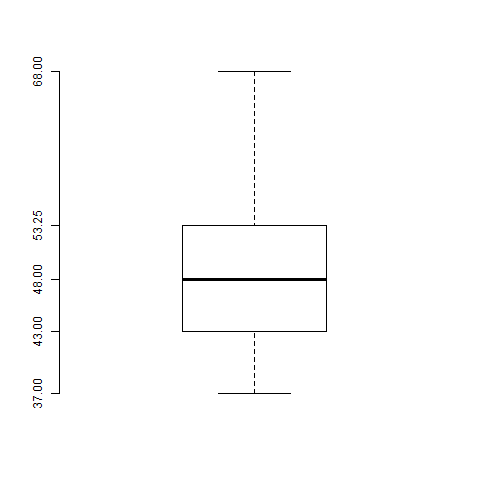
\includegraphics[width=0.9\textwidth]{extraTeX/appendix/TeX/ex3/boxplotEx2.png}
  \end{center}
    \captionof{figure}{ \label{fig:ex1.2} Boxplot Exercise 1.2 }
  \end{Figure}
\eocesol{
 (a)~Quantitative (discrete)
\newline
 (b)~ \begin{tabular}[t]{|*{7}{c|}}
\hline      0 & 1&  2 &  3  & 4  & 5  & 6 \\ 
\hline 7 &4 &6 &7 &4 & 4  & 8 \\
\hline 
    \end{tabular}
\newline
 (c)~The value 6. 
}%%%\end{problem}

\eocesol{
  
  (a)~The study variable is the moment of the day when emergency occurs. Qualitative nominal. 
 (b)~No, because it is a qualitative variable. \newline
 (c)~\begin{tabular}[t]{*{4}{c}}
 \hline   Afternoon   &  Morning  &    Night & Nonworking \\
  \hline       9       &  11  &         7  &         5 \\
\hline  0.2813   &  0.3438 &   0.2188 &   0.1563 \\
  \end{tabular}
\newline
 (d)~Fig.~\ref{fig:ex4}
  \begin{Figure}
  \begin{center}
    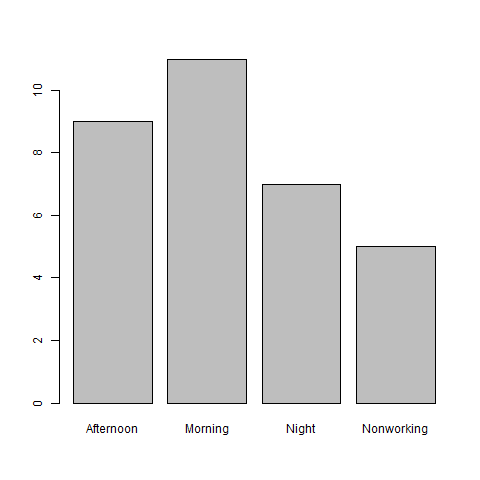
\includegraphics[width=0.9\textwidth]{extraTeX/appendix/TeX/ex3/barplotEx4.png}
  \end{center}  
\captionof{figure}{\label{fig:ex4} Bar plot exercise }
  \end{Figure}
}%%%}%%%\end{problem}
\eocesol{
  (a)  Copper levels in urine. Quantitative continuous
  (b) Median=0.71; Range=1.24-0.1=1.14
  (c) $Q_1=$0.5425; $Q_3=$0.8350  
  (d) 10-percentile=0.414  ; 95-percentile= 1.122
 (e) IQR=0.2925; Lower limit= 0.10375; Upper Limit= 1.27375; The value 0.1 is an outlying value 
 (f) Fig.~\ref{fig:ex5hist}  and \ref{fig:ex5box}  
}%%%\end{problem}

\begin{Figure}
 \begin{center}
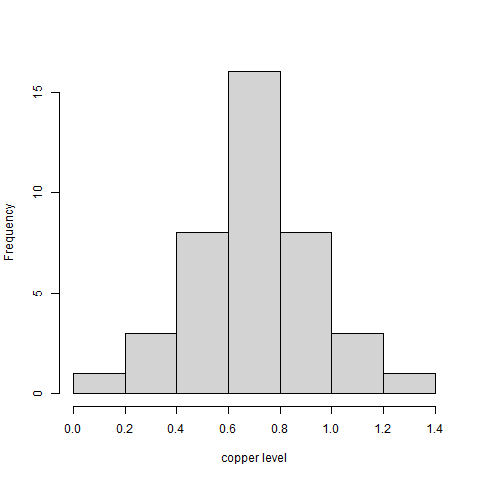
\includegraphics[width=0.9\textwidth]{extraTeX/appendix/TeX/ex3/histEx5.png} 
  \end{center}
  \captionof{figure}{\label{fig:ex5hist} Histogram Exercise 5}
\end{Figure}
\begin{Figure}
    \begin{center}
    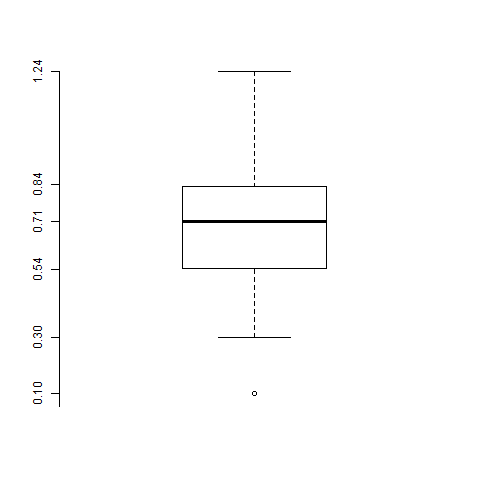
\includegraphics[width=0.9\textwidth]{extraTeX/appendix/TeX/ex3/boxplotEx5.png}
  \end{center}
  \captionof{figure}{\label{fig:ex5box} Boxplot}
\end{Figure}
\eocesol{
(a)~Qualitative continuous 
(b)~minimum and maximum; 3281 and  4422\newline 
 10 and 90 percentiles:3682.5 and 4288.0 ; \newline
 quartiles, median: $Q_1=$ 3955.75; $Q_2=$4125.00 $Q_3=$ 4173.00 \newline 
mean=4033.438\newline
mode ( It is not appropriate for a qualitative continuous variable) \newline range= 1141 \newline 
variance=82981.2, \newline 
standard deviation=288.0646
}%%%\end{problem}

\eocesolch{Probability and Distributions of Random Variables}


\eocesol{
 0.34+0.54-0.25=0.63
}%%%\end{problem}
\eocesol{
  (568-28)/568=540/568=0.9507
}%%%\end{problem}
\eocesol{
 $P(B\cap D)=0.15\cdot 0.24=0.036$
and $$P(B\cup D)=P(B)+P(D)-P(B\cap B)=0.15+0.24-0.036=0.354 $$
}%%%\end{problem}
\eocesol{
  Yes, because $P(A\cap B)=P(A)\cdot P(B)$
}%%%\end{problem}
\eocesol{
i) 0.4332; ii) 0.3445; iii) 0.9875; iv) 0.4920; v) 0.3174; vi) 0.2728;
vii) 0.0456; viii) 0.5886
  }
\eocesol{
  i)0.35; ii)1.54; iii) 2.16 iv) -1.24
}%%%\end{problem}
\eocesol{
  i)0.9970; ii) 0.0668 ; iii) 0.0873
}%%%\end{problem}
\eocesol{
  31.92\%
}%%%\end{problem}
\eocesol{
  95.44\%
}%%%\end{problem}
\eocesol{
The 80-percentile is 73.4. So, the answer is 
  74
}%%%\end{problem}
\eocesol{
 The lenght 6 feet is equivalent to 72 inches. \newline 
 $P(X<72)=P(Z<4/3)=0.9082$
}%%%\end{problem}
\eocesol{
  i)1.70\%; ii) 85.55
}%%%\end{problem}
\eocesol{
 i)  (3.08,10.92); ii) (2.34,11.66); iii) $(3.72,+\infty)$;\newline 
 iv) 4\%; 
v) 89.44\%; vi) 38.30\%; \newline 
vii) 9.19\% viii) 96 percentile
}%%%\end{problem}

\eocesol{
  i) (126.48,173.52); ii) (130.32,169.68); iii) (0,169.68) \newline
  iv) 74.86\%; v) 77.34\%; vi) 74.92\% ; vii) 98.12 percentile
}%%%\end{problem}
\eocesolch{Chapter 3}




%_______________

%% 4.1 SAMPLING VARIABILITY

% 1 oi_biostat, blue_eggs

\eocesol{(a)~$\overline{x} = 0.6052.$ \\
	(b)~$s = 0.0131$. \\
	(c)~$Z_{0.63} = \frac{0.63 - 0.6052}{0.0131} = 1.893$. No, this level of BGC is within 2 SD of the mean. \\
	(d)~The standard error of the sample mean is given by $\frac{s}{\sqrt{n}} = \frac{0.0131}{\sqrt{70}} = 0.00157$.
}

% There is not section with exercises\par
 \eocesolch{Chapter 4}


\eocesol{
 $80.5\pm 14.2\cdot 1.96 /\sqrt{24}$. The 95- CI is   $(74.8188,86.1812)$ 
}%%%\end{problem}
\eocesol{
$85=110(1-\alpha)$; $\alpha=0.15$; $1-\alpha/2=0.925$ and
$z_{0.925}=1.44$.

The error $z_{1-\alpha/2} \sigma /\sqrt{n}$ is less than $2.75$. Hence
$$n> z_{1-\alpha/2}^2\frac{\sigma^2 }{2.75^2}=1.44^2\frac{86.4}{2.75^2}=23.69$$  
  The sample size should be larger that 24. 
}%%%\end{problem}

\eocesol{
  $90\pm 1.96\cdot10/\sqrt{49}$. The 95-CI is $(87.2,92.8)$ 
}%%%\end{problem}

\eocesol{
  $\bar{x}=80.1333$ and $s=5.4099$. $t_{14,.975}=2.145$. \newline
$80.13\pm 2.145\cdot 5.4099/\sqrt{15}$ The 95-CI is
$(77.1371,83.1285)$. 
}%%%\end{problem}

\eocesol{
  $n=100>30$; $\bar{x}=23$; $s=10$; $100(1-\alpha)=90$; $\alpha=0.1$;
  $1-\alpha/2=0.95$; $ z_{.95}=1.64$ \newline 
$23\pm 1.64{\color{red} \cdot} 10/\sqrt{100}$. The 90\%-CI is $(21.36,24.64)$   
}%%%\end{problem}

\eocesol{
  Assuming that the weight of ten year-old male gorilla is a normal
  variable.

 $\alpha=0.1$ and $t_{24,.95}=1.711$

$36.5\pm 1.711{\color{red} \cdot} 5/\sqrt{25}$. The 90-CI is $(34.789,38.211)$.
}%%%\end{problem}

\eocesol{  %PROBLEM 7
 % $\bar{x}=12$; $n=10$; $s=7.7392$; $\alpha=0.05$; $t_{9,.975}=2.262$ 
 $\bar{x}=12$; $n=20$; $s=7.7392$; $\alpha=0.05$; $t_{19,.975}=2.093$ 

 $12\pm  2.093\cdot 7.7392/\sqrt{20}$. The 95\%-CI is $( 8.3780,15.6220)$
 }%%%\end{problem}

\eocesol{
  i)  $140\pm 1.96 \cdot 25 /\sqrt{200}$. The 95\%-CI  is
  $(136.5352,143.4648)$. \newline 
 ii)  There is an association between glaucoma and blood pressure,
 since the average blood pressure for glaucoma patients is higher than
 the general population.  
}%%%\end{problem}

\eocesol{
$\bar{x}=1.435$; $s=0.1461$, $t_{19,.975}=2.093$ \newline 
 $1.435 \pm 2.093\cdot 0.1461 /\sqrt{20}$.   The 95\%-CI is  $(1.3666,1.5034)$
}%%%\end{problem}

\eocesol{
 The question is about the confidence $100(1-\alpha)$.

The error $z_{1-\alpha/2} \sigma /\sqrt{n}$ is equal to 10 is 
$$z_{1-\alpha/2}=\frac{10}{\sigma}\sqrt{n}=10\frac{\sqrt{24}}{\sqrt{424}}=2.3792$$
$P(Z<2.38)=0.9913=1-\frac{\alpha}{2};$\qquad $\alpha=0.0174$; \qquad $100(1-\alpha)=98.26$
}%%%\end{problem}

% \eocesol{
% Confidence Interval of variance is not on the
% notes. \footnote{$((n-1)\frac{s^2}{\chi^2_{n-1,{\color{red}1-}\alpha/2}},((n-1)\frac{s^2}{\chi^2_{n-1,\alpha/2}})=(28\frac{34^2}{\chi^2_{28,0.95}},28\frac{34^2}{\chi^2_{28,0.05}})=(28\frac{34^2}{41.337},28\frac{34^2}{16.928})=(783.0273,1912.098)$ 
% }
%}%%%\end{problem}
\eocesol{\footnote{The number of
    positives outcomes is not greater than 10, so the interval
    calculated is not a very good approximation. }
  $\hat{p}=6/46$; $\frac{6}{46} \pm 1.96 \frac{\sqrt{(6/46)\cdot
     (40/46)}}{\sqrt{46}}$. The 95-CI is $(0.0331, 0.2278)$
}%%%\end{problem}

\eocesol{ % PROBLEM 13 
$\hat{p}=311/375$; $\frac{311}{375} \pm 1.64 \frac{\sqrt{(311/375)\cdot
     (64/375)}}{\sqrt{375}}$
 The  90-CI is  $(0.7975,0.8612)$. 
}%%%\end{problem}


%\eocesol{$^{\color{red}{\footnotemark}}$
 % One- year old cats:  $\hat{p}=6/21$; $\frac{6}{21} \pm 1.96 \frac{\sqrt{(6/21)\cdot
 %    (15/21)}}{\sqrt{21}}$. The 95-CI is $(0.0925,0.4789 )$\newline 
 %Two-year old cats:  $\hat{p}=12/16$; $\frac{12}{16} \pm 1.96 \frac{\sqrt{(12/16)\cdot
 %    (4/16)}}{\sqrt{16}}$. The 95-CI is $( 0.5378, 0.9622 )$
%}%%%\end{problem}

 \eocesolch{Chapter 5}

% \def\prob#1{\relax\par\noindent\textbf{Problem #1:}}


% Ejercicio eliminado por la la desviaci'on poblacional 
%\eocesol{ The test statistic is $z=\displaystyle\frac{13-14}{3.26}\sqrt{15}=-1.1880$. The
%p--value is $p=0.2348$. Hence, we fail to reject the null hypothesis. 
%}

\eocesol{
$t=\displaystyle\frac{9.77-7.65}{\sqrt{11.14}}\sqrt{15}=2.4600$. Acceptance
interval:$(-2.145, 2.145)$ Null Hypothesis is rejected. 
}
\eocesol{
$t=\displaystyle\frac{155.223-196.49}{88.04}\sqrt{27}=-2.4352$. 
Acceptance Interval: $(-2.056,2.056)$ Null
hypothesis is rejected. % $p=0.01102$.
}
\eocesol{%\prob{4}
(a)~$(24.29,25.71)$
(b)~The test statistic is $t=2.8207$. The p--value is
  $p=0.006583164$. (This value is calculated with R-Commander)
(c)~Null--Hypothesis is rejected. There is a statistically significant difference
  between the mean of body mass indeces of the diabetic and non
  diabetic population. 
(d)~ We know that the null hypothesis was going to be rejected
  because the value of the sample mean does not belong to the 95\%
  Confidence Interval. 
}
\eocesol{%\prob{5}
If we assume that blood pressure is normally distributed: 
\begin{enumerate}
\item The test statistic is $t=\displaystyle \frac{143-136}{24.4}\sqrt{86}=2.6605$  %1.1232
The acceptance region:
$(-t_{85,.95},t_{85,.95})=(-1.663,1.663)$. Null-hypothesis is rejected.
\item The test statistic is $t=\displaystyle \frac{87-84}{16.0}\sqrt{86}=1.738803$  %1.1232
 The acceptance region is the same than before. Now Null-hypothesis is
 rejected. 
\item There are enough statistical evidence in order to state that
  workers who have experienced a major coronary event have higher
  systolic and diastolic  blood pressure.
\end{enumerate}
 If normal distribution is not assumed, the statistic calculated is
approximately normal distributed because the sample is large enough
($>30$). Therefore, for the acceptance region
normal distribution and $(-1.645,1.645)$ and the conclusions are the
same. 
}
\eocesol{%\prob{6}
    Let $p$ be the proportion of solo practice for veterinary physician  
    \begin{align*}
      H_0: & p=0.43 & H_A:&p\neq 0.43 
    \end{align*}
  The data are sample proportion $\hat{p}=0.32$ and  sample size
  $n=223$.

The test statistic is 
$$z=
%\frac{\hat{p}-p}{\sqrt{\hat{p}(1-\hat{p})}/\sqrt{n}}=
\frac{0.32-0.43}{\sqrt{0.43(1-0.43)}/\sqrt{223}}=
-3.3180$$

The critical values for $\alpha=0.05$ are
$z_{1-\alpha/2}=z_{0.975}=1.96$ and $z_{\alpha/2}=-1.96$. The
acceptance region is $(-1.96,1.96)$. 

The  test statistic value does not belong to the acceptance region, the
null--hypothesis is  rejected. 

The p-value is 0.2726051
}


\eocesol{%\prob{7}
 $n=11$, sample mean $\bar{x}=69.3636$, sample variance
$s^2=39.6546$, sample standard deviation $s=6.2972$. 
Let $\mu$ be the mean value of the strength of the lateral digital extensor
muscle. 
\begin{align*}
      H_0: & \mu=65 & H_A:&\mu\neq 65 
    \end{align*}
The acceptance interval is $(-t_{10,.975},t_{10,.975})=(-2.228,2.228)$
and 
the test statistic is
$$t=\frac{69.3636-65}{6.2972/\sqrt{11}}=2.2982$$ 
The null hypothesis is rejected. There is enough evidence to state
that the mean mean value of the strength of the lateral digital extensor
muscle is different from 65.
}
\eocesol{%\prob{8}
 $p_0=0.25$, $n=125$, sample proportion $\hat{p}=35/125=0.28$.
\begin{align*}
      H_0: & p=0.25 & H_A:&p\neq 0.25 
    \end{align*}
The acceptance interval is $(-1.96,1.96)$ and the test statistic is
$$z=\frac{(0.28-0.25}{\sqrt{0.25\cdot 0.75}/\sqrt{125}}=0.7746$$
Null hypothesis is accepted. We don't have enough evidence to state
that the proportion is different from 25\%. 

p-value is 0.44.
}

\eocesol{%\prob{9} 
Acceptance interval
$(-t_{14,.975},t_{14,.975})=(-2.145,2.145)$ and test statistic is 
$$t=\frac{162.5-160}{5/\sqrt(15)}=1.9365$$
Null hypothesis is accepted. 
}
\eocesol{%\prob{10} 
 Sample size: $n=1500$, sample proportion
$\hat{p}=125/1500=0.0833$ \\
\textbf{Two--sided}: 
\begin{align*}
      H_0: & p=0.06 & H_A:&p\neq 0.06 
    \end{align*}
The acceptance interval is $(-1.96,1.96)$ and the test statistic is 
$$z=\frac{0.0833-0.06}{\sqrt{0.06\cdot 0.94}/1500}=3.7998$$
Null hypothesis is rejected.  \\
p--value$= 2(1-Pr(Z<3.80))=2(1-0.9999)=0.0002$ \\
\textbf{One--sided}:
\begin{align*}
      H_0: & p=0.06 & H_A:&p> 0.06 
    \end{align*}
The acceptance interval is $(-\infty,1.64)$ and the test statistic is
the same value
$$z=3.7998$$
Null hypothesis is rejected. 
p--value$= 1-Pr(Z<3.80)=1-0.9999=0.0001$
}
\eocesol{Sample size: $n=150>30$. With $\alpha=0.05$ the acceptance
interval is $(-1.96,1.96)$ and $z=\frac{325-332}{52/\sqrt{150}}=-1.6487$ 
}
\eocesolch{Chapter 6}



\eocesol{%\prob{1} 
Sample proportions: $\hat{p}_1=0.2333$ $\hat{p}_2=0.32$. Pool
proportion: $\hat{p}=0.2727$. \newline 
Test statistic: $z=2.7831$. Acceptance interval: $(-1.96,1.96)$
\newline 
Null hypothesis is rejected. 
}

\eocesol{%\prob{2} 
Sample proportions: $\hat{p}_1=0.58$ $\hat{p}_2=0.5294$. Pool
proportion: $\hat{p}=0.5531$. \newline 
Test statistic: $z= -0.9083$.  p--value= $2\cdot
(1-Pr(Z<0.91))=2\cdot(1-0.8186)= 0.3628$  \newline 
Null hypothesis is accepted. 
}
\eocesol{%\prob{3} 
Sample proportions: $\hat{p}_1=0.0704$ $\hat{p}_2=0.0562$. Pool
proportion: $\hat{p}=0.0619.$. \newline  Test statistic:$z= -1.6688$.
p--value $2\cdot (1-Pr(Z<1.67))=2\cdot (1-0.9525)=0.095$.\newline 
Null hypothesis is accepted
}
\eocesol{%\prob{4} 
  The same calculation than problem 3.
}
\eocesol{ %\prob{5}
 i) $F=1.0808$ Acceptance interval
$(F_{11,8,.025},F_{11,8,.975})$. We don't have the value
$df_1=11$. So, we  use $df_1=10$ (or $df_1=12$). 
$(F_{10,8,.025},F_{10,8,.975})=(1/3.85,4.30)=(0.26,4.30)$. Null
hypothesis is accepted. \newline
ii) $S_p^2=(11\cdot 1.05^2 + 8\cdot 1.01^2)/19=1.0678$. Test statistic
$t= 4.8500$. Acceptance interval
$(-t_{19,.975},t_{19,.975})=(-2.093,2.093)$. Null hypothesis rejected.  
}
\eocesol{%\prob{6} 
 $\bar{x}_1-\bar{x}_2=3.4125$ y  $s_{x_1-x_2}=3.6443$.
Test statistic $t=2.6485$. Acceptance interval:
$(-t_{7,.975},t_{7,.975})=(-2.365,2.365)$. \newline 
Null hypothesis is rejected.
}
\eocesol{  %\prob{7} 
i) Test statistic: $F=1.1475$. Acceptance interval:
$(0.36.2.57)$. Assume equal variances. \newline 
ii) $S^2_p=12.9714$. Test statistic: $ t= 2.0917$. Acceptance
interval:$(-2.030,2.030)$ . Reject null hypothesis \newline 
iii) p-value is 0.0437  using R-Commander. 
}
\eocesol{%\Prob{8}
Test equal Variances. Test statistic: $F=35.5^2/37.6^2=0.8914$. Acceptance interval
$(F_{24,46,.025},F_{24,46,.975})$. We use degree of freedom 25 and 50
, $(1/2.08,1.92)=(0.48,1.92)$. Hence, null hypothesis is accepted. 

Test means: $S_p^2=  1312.882$. Test statistic:   $-0.02869$. Acceptance
interval $(-t_{70,.975}, t_{70,.975})=(-1.994,1.994)$. Null hypothesis
is accepted.
}
\eocesolch{Chapter 7}
 \eocesol{1. There is not outlying values, so we could assume the distribution to be normal. Variability is similar across groups. 2. All the p-values are greater to 0.05, conditions to apply ANOVA could be assume according to these tests. 3. (a) Snedecor's F distribution. (b)  [0, 3.09) (c) No, ANOVA is not used to identify which pairs are different. 4. There are significant difference for any pair of comparisons since 0 is not included-}
 \eocesol{(a) Yes, (b) $H_0:\mu_A=\mu_B=\mu_C$ and $H_1:\mu_A\neq\mu_B \text{ or } \mu_A\neq\mu_C \text{ or }\mu_B\neq\mu_C$ 4. We have evidence that $A$ is different from $B$ and $C$.} 
 \eocesol{ With $\alpha=0.05$ we do noy have evidence of difference across sections. }
 \eocesol{(a)~$H_0$: Average GPA is the same for all majors. $H_A$: At least one pair of means are different.
	(b)~Since p-value $>$ 0.05, fail to reject $H_0$. The data do not provide convincing evidence of a difference between the average GPAs across three groups of majors.
	(c)~The total degrees of freedom is $195 + 2 = 197$, so the sample size is $197+1=198$.}
\eocesolch{Chapter 8}
\eocesol{ $x^2=61.356$; Rejection interval: $(5.99,+\infty)$ 
}
\eocesol{
$x^2=0.76536$; Rejection interval: $(7.81,+\infty)$
}
\eocesol{$x^2=0.82589$; ; Rejection interval: $(5.99,+\infty)$ 
}
\eocesol{$x^2=50.323$ ; Rejection interval: $(9.21,+\infty)$}
\eocesol{$x^2=4.71$;  Rejection interval: $(3.841,+\infty)$}
 \end{multicols}
\include{extraTeX/appendix/TeX/vetTables}
%\include{extraTeX/appendix/TeX/zTable}
%\include{extraTeX/appendix/TeX/tTable}
%\include{extraTeX/appendix/TeX/chiSquareTable}
\endgroup

\cleardoublepage
\addcontentsline{toc}{chapter}{Index}
\printindex

\end{document}
